\documentclass[a4paper,11pt]{article}
\usepackage[T1]{fontenc}
\usepackage[utf8]{inputenc}
\usepackage{lmodern}
\usepackage[francais]{babel}
\usepackage{geometry}
\usepackage{float}
\usepackage{array}
\usepackage{multirow}
\usepackage{makecell}
\usepackage{graphicx}
\usepackage{listings}


\newcolumntype{M}[1]{>{\raggedright}m{#1}}

\geometry{hmargin=2.5cm,vmargin=2.5cm}

\title{Logique floue\\\texttt{Sauvons le RMS Titanic}}

\author{Alexis \textsc{Decker-Wurst}, Erwan  \textsc{Duroux}, Guillaume  \textsc{Laroyenne}}

\begin{document}

    \maketitle

    \begin{abstract}
        Ce document présente une synthèse du projet de logique floue que nous avons réalisé en deuxième année.\\
        Le cœur de ce projet est une bibliothèque de logique floue que nous avons programmé en \textit{C++}. La bibliothèque comporte les principaux opérateurs de bases de la logique floue ainsi que quelques méthodes de défuzzification.\\
        Pour les utilisateurs puissent manipuler plus simplement cette bibliothèque, nous avons décidé d'ajouter un interpréteur permettant de modéliser des problèmes de logique floue sans avoir à la manipuler directement.\\
        La logique floue permettant de prendre des décisions complexe à partir d'un ensemble de données. Nous avons décidé de l'utiliser afin de réaliser un pilote automatique évitant les obstacles pouvant se trouver devant un navire, tout en utilisant la bibliothèque que nous avons conçu.
    \end{abstract}

    \section{Construction de la bibliothèque de logique floue}

    \begin{figure}[h!]
        \begin{center}
            \caption{UML des packages du \texttt{Framework}}
            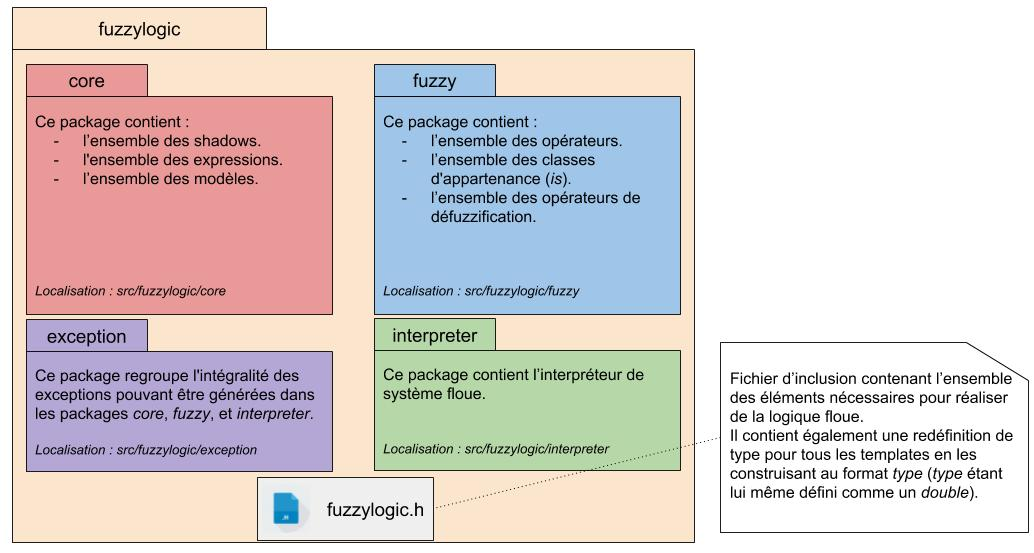
\includegraphics[scale=0.5]{assets/Packages_(UML).jpg}
            \label{fig:umlPackage}
        \end{center}
    \end{figure}


    \begin{table}[h!]
        \caption{Liste des opérateurs est opérandes du \textit{Framework}}
        \label{tab:listing}

        \begin{center}
            \begin{tabular}{|c|c|M{4cm}|}
                \hline
                Nom & Type & Description \tabularnewline
                \hline
                court texte & truc & Texte plus long qui sera centré dans la ligne et aligné à gauche dans la colonne  \tabularnewline
                \hline
            \end{tabular}
        \end{center}
    \end{table}
    
    \section{Mise en place d'un interpréteur de logique floue}


    \begin{figure}[h!]
        \begin{center}
            \caption{Schéma présentant le concept de l'interpreteur}
            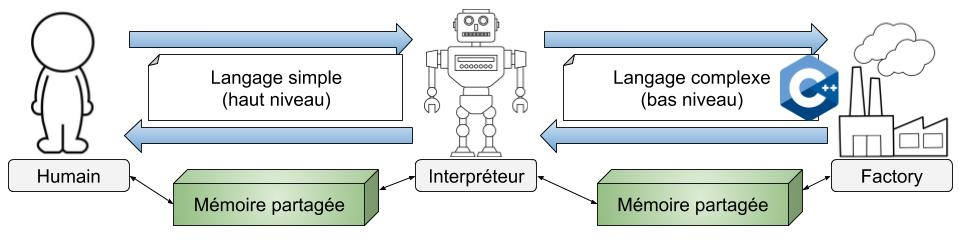
\includegraphics[scale=0.5]{assets/Interpreteur_Dessin.jpg}
            \label{fig:interpreterDessin}
        \end{center}
    \end{figure}

    \begin{figure}[h!]
        \begin{center}
            \caption{Exemple de code de l’interpréteur pour l’évaluation d'un pourboire}
            \lstinputlisting[language=Bash, firstline=0, lastline=9, frame=single]{assets/leaveatip_cog.fuzzy}
            \label{fig:codeExemple}
        \end{center}
    \end{figure}

    \section{Création du simulateur naval}

    \begin{figure}[h!]
        \begin{center}
            \caption{Schéma présentant les forces physique appliquées sur le Titanic dans le simulateur}
            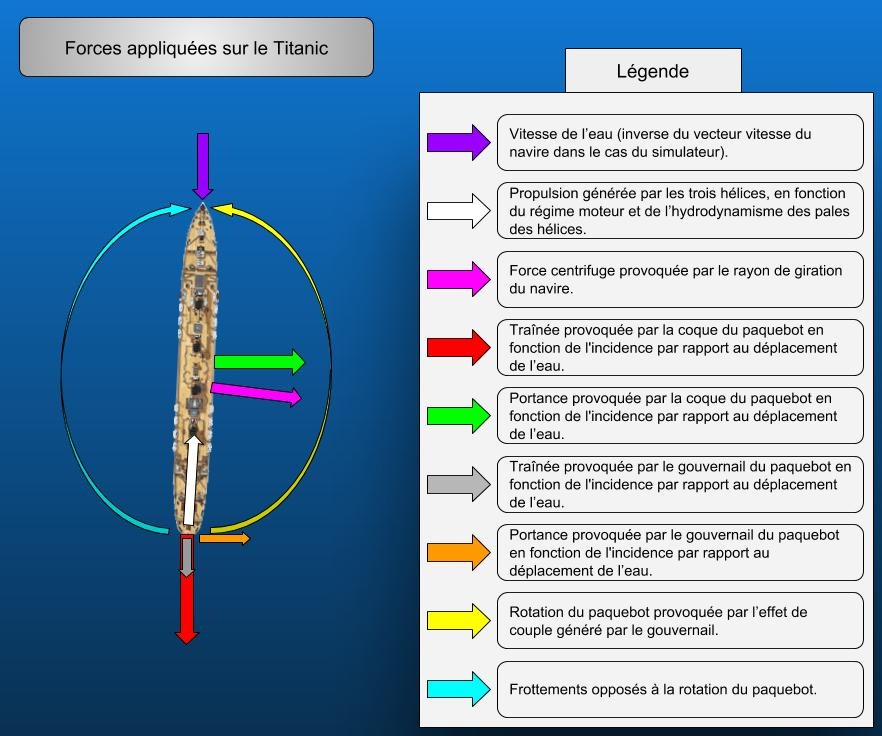
\includegraphics[scale=0.5]{assets/Isaac_vs_Titanic.jpg}
            \label{fig:titanicForces}
        \end{center}
    \end{figure}

    \section{Création d'un pilote automatique pour le paquebot}

    \subsection{Objectifs et besoins}

    Le pilote automatique doit permettre au Titanic d’éviter les icebergs en toute sécurité avant même que l'équipage puisse les voir.
    Mais pour éviter les icebergs, il est nécessaire de les détecter. Pour cela nous avons ajouté à la proue trois capteurs lasers indiquant une distance en pourcentage par rapport à sa portée.
    Si un capteur indique 100\% alors il n'y a pas d'objet. En revanche si un capteur indique 50\% alors il y a un objet à la moitié de la potée maximal du capteur. Les trois lasers ont été placé avec un petit angle, afin de pouvoir déterminé le meilleur côté par le quel l'objet peut être évité.

    \begin{figure}[h!]
        \begin{center}
            \caption{Schéma présentant les capteurs lasers du Titanic}
            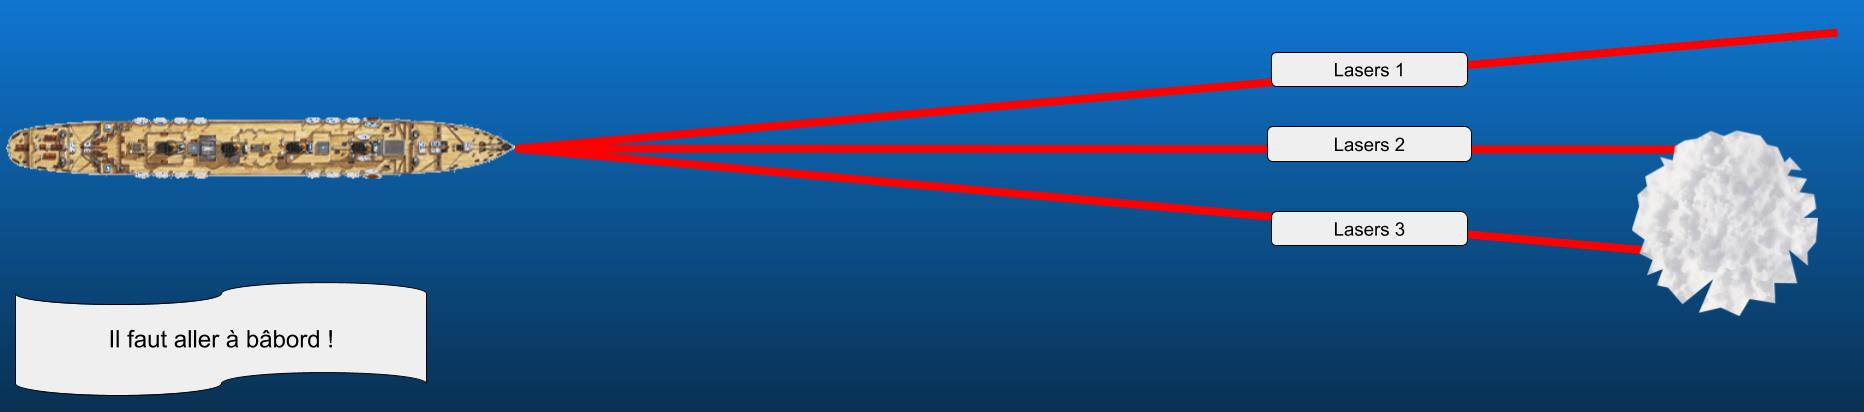
\includegraphics[scale=0.26]{assets/Lasers_Illustration.jpg}
            \label{fig:titanicLasers}
        \end{center}
    \end{figure}

    Pour déterminer la meilleur portée des lasers, il faut connaître la capacité a virer de bord du navire. Dans les meilleurs conditions, le Titanic avait un rayon de giration de 750 m. Nous avons donc réglé la portée des lasers à 800 m, ce qui devrait permettre d’anticiper l’approche des objets suffisamment tôt.

    \subsection{Modélisation du pilote automatique en logique floue}

    \subsection{Réalisation du système floue à l'aide du \textit{framework}}

    \begin{figure}[h!]
        \begin{center}
            \caption{Code du pilote automatique pour l’interpréteur}
            \lstinputlisting[language=Bash, firstline=0, lastline=10, frame=single]{assets/automatic-pilot.fuzzy}
            \label{fig:codeAutoPilot}
        \end{center}
    \end{figure}

\end{document}
